% ============================================
% PÁGINA 1: PORTADA FUUL PAGE
% ============================================
\begin{titlepage}
    \thispagestyle{empty}
    \pagestyle{empty}
    
    % 1. Elimina todos los márgenes para esta página
    \newgeometry{margin=0cm}
    
    % 2. Imagen a tamaño físico del papel
    \noindent
    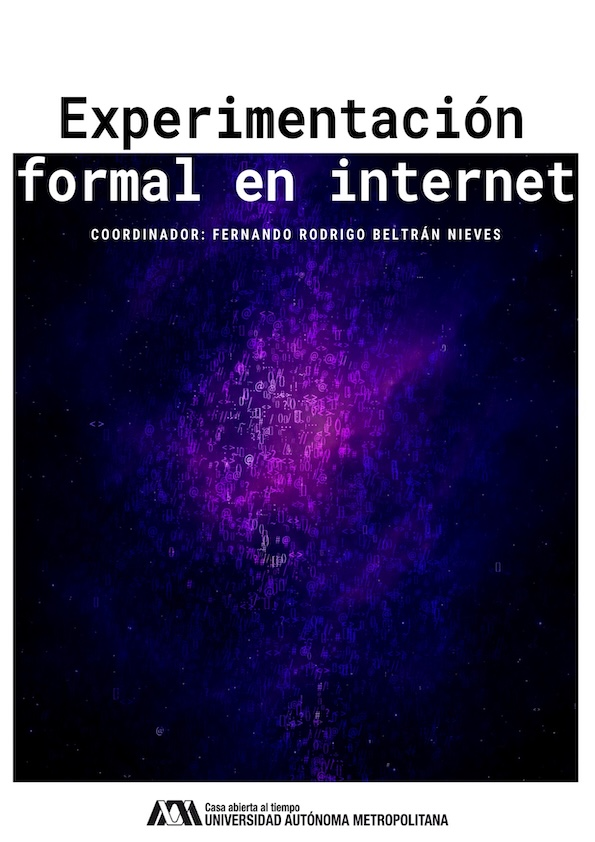
\includegraphics[width=\paperwidth, height=\paperheight, keepaspectratio]{assets/imagenes/portada.jpeg}
    
    % 3. Cierra página y restaura márgenes para el resto del libro
    \clearpage
    \restoregeometry
\end{titlepage}
% ============================================
% PÁGINA 2: EN BLANCO (verso de portada)
% ============================================
\clearpage
\thispagestyle{empty}
\null
\clearpage

% ============================================
% PÁGINA 3: PORTADILLA (MEDIA PORTADA)
% ============================================
\clearpage
  \thispagestyle{empty}
  \pagestyle{empty}
  
  % INICIO DEL ALINEAMIENTO IZQUIERDO (solo para esta página)
  \begingroup  % ← Inicia grupo local
    \raggedright
      \vspace*{1.5cm}
      {\LARGE \textbf{Experimentación formal en internet \\(o de cómo las Ciencias Sociales habitan la galaxia)}} \\
      \vspace{0.3cm}
      {\large Convergencias, algoritmos y narrativas emergentes} \\
      \vspace{1cm}
      {\LARGE Fernando Rodrigo Beltrán Nieves} \\
      \vspace{0.3cm}
      {\large Coordinador}
      
      \vfill
      
      \begin{minipage}[t]{0.50\textwidth}
          \includegraphics[width=1.5\textwidth]{../../assets/logos/logo_uam_l.png}
      \end{minipage}
  \endgroup  % ← TERMINA EL GRUPO: restaura justificación automática
\clearpage

% ============================================
% PÁGINA 4: CRÉDITOS / DATOS LEGALES
% ============================================
\begin{titlepage}
    \thispagestyle{empty}
    \vspace*{2cm}

    \normalfont
    \centering
        \textbf{Experimentación formal en internet \\ (o de cómo las Ciencias Sociales habitan la galaxia)} \\
        \textit{Convergencias, algoritmos y narrativas emergentes} \\
        \vspace{0.5cm}
        \small
        Coordinador: Fernando Rodrigo Beltrán Nieves \\
        Universidad Autónoma Metropolitana \\
        Unidad Lerma \\
        
        
        \rule{0.6\textwidth}{0.4pt}
        \vspace{0.5cm}
        
        \small
        \textbf{Datos de catalogación} \\
        \vspace{0.3cm}
        Primera edición, 2026 \\
        Lerma de Villada, Estado de México \\
        \vspace{0.3cm}
        ISBN: 978-xxx-xxx-xxx-x \\
        D.R. © 2026, Universidad Autónoma Metropolitana \\
        Unidad Lerma \\
        Av. Hidalgo Poniente 46, Col. La Estación, \\
        Lerma de Villada, Estado de México, C.P. 52006 \\
        \vspace{0.3cm}
        Impreso y hecho en México \\
        \vspace{0.3cm}
        Queda prohibida la reproducción total o parcial \\
        sin autorización escrita del titular de los derechos

\end{titlepage}

% ============================================
% REGRESO A ESTILO NORMAL
% ============================================
\clearpage
\pagestyle{headings}  % ← Restaura encabezados con nombre de capítulo
\setcounter{page}{1}